\documentclass[aspectratio=169,11pt]{beamer}
\usetheme{Madrid}
\usecolortheme{seahorse}
\setbeamertemplate{navigation symbols}{}
\usepackage[T1]{fontenc}
\usepackage{lmodern}
\usepackage{booktabs}
\usepackage{array}
\usepackage{xcolor}
\usepackage{listings}
\usepackage{amsmath}
\usepackage{amssymb}
\usepackage{tikz}
\usetikzlibrary{arrows.meta,positioning}

\newcommand{\code}[1]{\texttt{\detokenize{#1}}}
\newcommand{\NaN}{NaN}
\definecolor{nanred}{RGB}{214,39,40}
\definecolor{validblue}{RGB}{31,119,180}
\definecolor{padgray}{RGB}{150,150,150}
\definecolor{maskdark}{RGB}{60,60,60}
\lstset{basicstyle=\ttfamily\scriptsize, columns=fullflexible, keepspaces=true, breaklines=true,
        backgroundcolor=\color{black!4}, frame=single, rulecolor=\color{black!15}, language=C++,
        escapeinside={(*@}{@*)}}

\title[Flash padding lanes]{Flash Attention, Padding Lanes, and\\ \texttt{lse\_sum != lse\_sum}}
\subtitle{A controlled study of the NaNs nixnan reports in PyTorch's flash kernels}
\author[SC26 nixnan tutorial]{SC26 nixnan tutorial}
\institute[]{\texttt{flash-attn-expt}, branch \texttt{Flash-Attn}}
\date{October 2026}

\begin{document}

\begin{frame}
\titlepage
\end{frame}

%-----------------------------------------------------------------------------
\begin{frame}{The question}
\begin{itemize}
\item nixnan on \textbf{BioMistral-7B} (4-bit NF4, HF + SDPA): millions of \NaN/$\pm\infty$/subnormal operands
  \begin{itemize}
  \item mostly in \code{pytorch_flash::flash_fwd_kernel}: \code{HMMA.16816.F32} op 2, \code{FADD [NaN,subnormal]}
  \item almost nothing reaches memory
  \end{itemize}
\item Three candidate explanations:
\end{itemize}
\vspace{2mm}
\begin{columns}[T]
\begin{column}{0.32\textwidth}
\begin{block}{H1: flash's guards}\small
Flash filters \NaN{} on purpose, e.g.\ in the combine kernel:\\
\code{(lse_sum == 0 || lse_sum != lse_sum)}
\end{block}
\end{column}
\begin{column}{0.32\textwidth}
\begin{block}{H2: 4-bit}\small
nixnan misreads packed NF4 weights as FP16/FP32 operands
\end{block}
\end{column}
\begin{column}{0.32\textwidth}
\begin{block}{H3: padding lanes}\small
Fixed $128\times128$ tiles; rows/cols outside the sequence are never loaded or cleared
\end{block}
\end{column}
\end{columns}
\end{frame}

%-----------------------------------------------------------------------------
\begin{frame}{Test bed: TinyGPT on the same flash binaries}
\begin{columns}[T]
\begin{column}{0.52\textwidth}
\begin{itemize}\small
\item Decoder-only, digits 0--9, 4 layers, $d=128$, 4 heads $\times$ 32, RoPE
\item 100 random training words (\code{training-set.txt}); loss 0.3939 (optimum 0.3938)
\item FP32 linears (no tensor cores); attention FP16 via SDPA, \textbf{flash forced}
\item Same venv as BioMistral: torch 2.6.0+cu124, bitsandbytes 0.48.1
\item Task: \code{312} $\to$ \code{312452} (3 forward passes $\times$ 4 layers = 12 flash calls)
\item A/B: 301-key prompt (2 KV splits) + an \emph{external input} on the last embedding: A = 0, B = $+\infty$
\end{itemize}
\end{column}
\begin{column}{0.45\textwidth}
\begin{block}{Two lenses}\small
\textbf{1. nixnan} (NVBit): training at \code{SAMPLING=32}, inference fully monitored, kernel whitelists\\[2mm]
\textbf{2. Source instrumentation}: PyTorch 2.6's own flash source, recompiled with dump hooks, \textbf{bitwise-equal} to PyTorch's kernel
\end{block}
\end{column}
\end{columns}
\end{frame}

%-----------------------------------------------------------------------------
\begin{frame}{Lens 1 --- nixnan: clean data reproduces BioMistral, 4-bit is innocent}
\small
\resizebox{\linewidth}{!}{%
\begin{tabular}{@{}lll@{}}\toprule
run & \code{SAMPLING} & nixnan result\\\midrule
completion \code{312}$\to$6, every real tensor finite & 0 & \code{flash_fwd_kernel}: \textbf{1{,}183 FP32 + 184 FP16 \NaN{} sites}\\
NF4 linears (\code{kDequantizeBlockwise}, \code{kgemm_4bit}\dots) & 0 & bitsandbytes: \textbf{0 \NaN/Inf}, 19 subnormal sites\\
FP16 linears (cuBLAS/CUTLASS) & 0 & 41 subnormal reports, 0 \NaN/Inf\\
training, 1{,}500 steps & 32 & fwd: 1{,}493 sites; bwd: 458 sites, \textbf{no \NaN}\\
prompt length $T\le16$ / $T\ge32$ & 0 & 300--930 \NaN{} sites / \textbf{0}\\
same $T=16$ run, three times & 0 & 681, 930, 937 sites\\\bottomrule
\end{tabular}}
\vspace{3mm}
\begin{itemize}
\item Irregular in $T$, different on every repeat $\Rightarrow$ looks like \textbf{uninitialized memory}
\item nixnan's \code{INSTR_MEM} skips all of flash's stores (packed FP16 \code{STG.E.128}) $\Rightarrow$ ``no \NaN{} in memory'' is not evidence
\item nixnan says \emph{which instruction}, not \emph{which lane}
\end{itemize}
\end{frame}

%-----------------------------------------------------------------------------
\begin{frame}{Getting nixnan to run on PyTorch at all}
\begin{itemize}
\item First direct runs: never past start-up (20+ min, 27 GB RSS). Three causes:
\end{itemize}
\vspace{2mm}
\begin{columns}[T]
\begin{column}{0.32\textwidth}
\begin{block}{Instrumentation cost}\small
NVBit spends $\approx$30\,s per new cuBLAS/CUTLASS kernel.\\[1mm]
Fix: \code{FUNCTION_WHITELIST} (full demangled names; a full tile is a different template instance, so log names first with a dummy whitelist)
\end{block}
\end{column}
\begin{column}{0.32\textwidth}
\begin{block}{Hangs}\small
\code{F.embedding} hangs NVBit at load, even uninstrumented; so does the CUB radix sort in \code{weight[idx]}'s backward.\\[1mm]
Fix: embedding as \code{one_hot(idx) @ W} (bit-identical)
\end{block}
\end{column}
\begin{column}{0.32\textwidth}
\begin{block}{\texttt{LD\_PRELOAD} scope}\small
\code{LD_PRELOAD=nixnan.so timeout ...} instruments \code{timeout} too: two writers, one \code{LOGFILE}.\\[1mm]
Fix: \code{timeout N env LD_PRELOAD=... python}
\end{block}
\end{column}
\end{columns}
\vspace{3mm}
\small Result: completion fully monitored in seconds; training (1{,}500 steps, \code{SAMPLING=32}) in 57 min.
\end{frame}

%-----------------------------------------------------------------------------
\begin{frame}[fragile]{Lens 2 --- instrumenting PyTorch's flash source}
\begin{columns}[T]
\begin{column}{0.55\textwidth}
\small
\begin{itemize}
\item Copy of \code{aten/.../cuda/flash_attn} (v2.6.0)
  \begin{itemize}\footnotesize
  \item namespace renamed \code{instr_flash}; FP16 hdim-32 kernels only
  \item host side = PyTorch's own \code{mha_fwd} (same split heuristic, tiles)
  \end{itemize}
\item Hooks (\code{instrumentation.patch}):
  \begin{itemize}\footnotesize
  \item \code{flash_fwd_kernel}: whole tiles: \code{sQ sK sV} (raw FP16 bits), $S$, $S$ masked, $P$, $O$, per-row \code{softmax.h} guard
  \item split kernel: guard per (split, head, row)
  \item combine: \code{lse_sum}, both disjuncts, replaced/stored value, \NaN{} in $O$
  \end{itemize}
\item \textbf{16/16 bitwise equal} to \code{aten::_scaled_dot_product_flash_attention} (dumps on and off)
\end{itemize}
\end{column}
\begin{column}{0.43\textwidth}
\begin{lstlisting}
template <typename TensorS> __device__
void instr_dump_smem(float *dst,
                     TensorS const &s, int R, int C) {
  for (int i = threadIdx.x; i < R*C;
       i += blockDim.x)
    dst[i] = float(s(i / C, i % C).raw());
}
// ... in the masking loop:
if (instr_on && masking_step == 0) {
  instr_dump_smem(dst + dbg::Q, sQ, 128, 32);
  instr_dump_smem(dst + dbg::K, sK, 128, 32);
}
\end{lstlisting}
\footnotesize Fast math off: with \code{--use_fast_math} the combine LSE is 1 ulp off.
\end{column}
\end{columns}
\end{frame}

%-----------------------------------------------------------------------------
\begin{frame}{The padding lanes, dumped (last decode step, $s_q=1$, $s_k=6$)}
\begin{columns}[c]
\begin{column}{0.55\textwidth}
\centering
\setlength{\tabcolsep}{2pt}
\begin{tabular}{cccc}

\includegraphics[height=0.34\textheight,interpolate=false]{figs/tile_Q.png} &

\includegraphics[height=0.34\textheight,interpolate=false]{figs/tile_K.png} &

\includegraphics[height=0.34\textheight,interpolate=false]{figs/tile_S_RAW.png} &

\includegraphics[height=0.34\textheight,interpolate=false]{figs/tile_P.png}\\
\scriptsize sQ & \scriptsize sK & \scriptsize $S=QK^\top$ & \scriptsize $P$
\end{tabular}\\[2mm]
\textcolor{validblue}{\rule{1.2ex}{1.2ex}} in sequence \;
\textcolor{padgray}{\rule{1.2ex}{1.2ex}} finite pad \;
\textcolor{nanred}{\rule{1.2ex}{1.2ex}} \NaN \;
\textcolor{maskdark}{\rule{1.2ex}{1.2ex}} $-\infty$ (mask)
\end{column}
\begin{column}{0.43\textwidth}
\scriptsize
\begin{tabular}{@{}lrr@{}}\toprule
call 11, 4 heads & values & \NaN\\\midrule
Q row 0 (loaded) & 128 & 0\\
\textbf{Q rows 1--127 (never loaded)} & 16{,}256 & \textbf{3{,}239}\\
$S$ valid (row 0, keys 0--5) & 24 & 0\\
\textbf{$S$ padding rows} & 65{,}024 & \textbf{18{,}274}\\
\textbf{$P$ padding rows} & 65{,}024 & \textbf{798}\\
\textbf{$O$ padding rows} & 16{,}256 & \textbf{4{,}256}\\
$O$ row 0 (the output) & 128 & 0\\\bottomrule
\end{tabular}\\[2mm]
\small
\begin{itemize}
\item \textbf{Every \NaN{} lies outside the sequence}
\item \code{softmax.h}'s \code{sum != sum} fires on 133 padding rows; their LSE and $O$ are never stored
\end{itemize}
\end{column}
\end{columns}
\end{frame}

%-----------------------------------------------------------------------------
\begin{frame}{Where the garbage comes from: the previous launch's output}
\begin{columns}[c]
\begin{column}{0.57\textwidth}
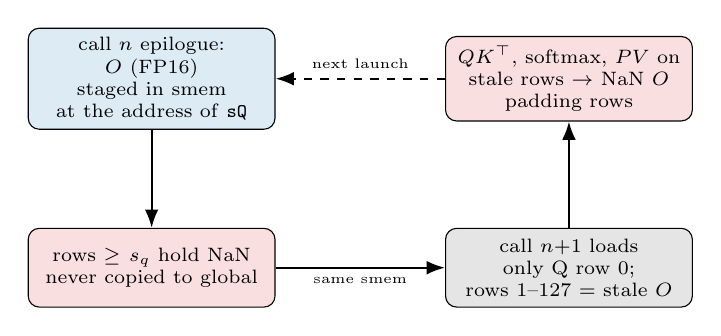
\begin{tikzpicture}[font=\scriptsize, box/.style={draw, rounded corners, text width=2.9cm, minimum height=1.0cm, align=center}]
\node[box, fill=validblue!15] (a) at (0,2.4) {call $n$ epilogue:\\$O$ (FP16) staged in smem\\at the address of \code{sQ}};
\node[box, fill=nanred!15] (b) at (0,0) {rows $\ge s_q$ hold \NaN{}\\never copied to global};
\node[box, fill=padgray!25] (c) at (5.3,0) {call $n{+}1$ loads only Q row 0;\\rows 1--127 = stale $O$};
\node[box, fill=nanred!15] (d) at (5.3,2.4) {$QK^\top$, softmax, $PV$ on\\stale rows $\to$ \NaN{} $O$\\padding rows};
\draw[-{Latex}, thick] (a) -- (b);
\draw[-{Latex}, thick] (b) -- node[below, font=\tiny]{same smem} (c);
\draw[-{Latex}, thick] (c) -- (d);
\draw[-{Latex}, thick, dashed] (d) -- node[above, font=\tiny]{next launch} (a);
\end{tikzpicture}
\end{column}
\begin{column}{0.41\textwidth}
\small
\begin{itemize}
\item \textbf{416 of 508} stale Q rows are bit-identical to rows of the previous call's $O$ tile
\item Call $n$'s 130 \NaN{} $O$ rows $\to$ call $n{+}1$'s 130 \NaN{} Q rows
\item Stale K rows: zeros or old K rows
\item Second identical run: \textbf{different} stale tiles, \textbf{bitwise-identical} output
\end{itemize}
\vspace{1mm}
\footnotesize Source: ``We don't need to clear the sQ smem tiles since we'll only write out the valid outputs''
\end{column}
\end{columns}
\end{frame}

%-----------------------------------------------------------------------------
\begin{frame}{The guards, dumped: inputs A (clean) and B ($+\infty$)}
\begin{columns}[T]
\begin{column}{0.55\textwidth}
\scriptsize
\resizebox{\linewidth}{!}{%
\begin{tabular}{@{}lrr@{}}\toprule
12 calls, 4 heads & A & B\\\midrule
split \code{softmax.h}, real rows: \code{sum != sum} $\to-\infty$ & 0 & \textbf{1{,}144}\\
split \code{softmax.h}, padding rows: \code{sum != sum} & 1{,}588 & 3{,}931\\
combine guard fired (real rows) & 0 & \textbf{568}\\
\quad via \code{lse_sum == 0} & 0 & 568\\
\quad via \textbf{\code{lse_sum != lse_sum}} & \textbf{0} & \textbf{0}\\
output rows with \NaN & 0 & \textbf{752}\\
completion & \code{..312489} & \code{..312000}\\\bottomrule
\end{tabular}}
\end{column}
\begin{column}{0.43\textwidth}
\small
\begin{itemize}
\item \NaN{} is removed one level earlier: \code{softmax.h} turns a \NaN{} sum into $\mathrm{lse}_s=-\infty$
\item Combine sees only finite/$-\infty$; all $-\infty$ $\Rightarrow$ \code{lse_sum = 0}
\item \textbf{The guard cleans the LSE, not $O$}: $0\cdot\NaN$ in $O \mathrel{+}= e^{\ldots}O^{\mathrm{acc}}_s$
\item Causality broken by tiling: rows 256--300 share the poisoned split
\end{itemize}
\end{column}
\end{columns}
\end{frame}

%-----------------------------------------------------------------------------
\begin{frame}[fragile]{Why \texttt{lse\_sum != lse\_sum} cannot fire for a positive scale}
\begin{columns}[T]
\begin{column}{0.56\textwidth}
\small
\begin{itemize}
\item \code{lse_sum} is \NaN{} $\iff$ some $\mathrm{lse}_s\in\{\NaN,+\infty\}$ ($\infty-\infty$)
\item $\mathrm{lse}_s = (\ell{=}0 \lor \ell{\ne}\ell)\,?\,-\infty : m\sigma+\log\ell$\\
  $\Rightarrow$ needs $\ell=+\infty$
\item Term $=2^{\,\mathrm{fl}(x\sigma_2)-\mathrm{fl}(m\sigma_2)}$, $x\le m$:
  \begin{itemize}\footnotesize
  \item $\mathrm{fl}(m\sigma_2)$ finite: terms $\in[0,1]$, $\ell\in[1,s_k]$
  \item overflow: max element gives $\infty-\infty=\NaN$ $\to$ guard $\to-\infty$
  \end{itemize}
\item \textbf{Proposition}: $\sigma>0$ $\Rightarrow$ unreachable for \emph{every} FP16 input (incl.\ $\pm\infty$, \NaN)
\item TinyGPT ($1/\sqrt{32}$), BioMistral ($1/\sqrt{128}$): \textbf{impossible}
\end{itemize}
\end{column}
\begin{column}{0.42\textwidth}
\footnotesize Source: \code{exp2f(x * scale - max_scaled)}\\ ``allows the compiler to use the ffma instruction'' --- \textbf{it doesn't}:
\begin{lstlisting}
FMUL R28, R28, c[0x0][0x238] ;
...
FADD R154, -R47, R154 ;
FSETP.GEU.AND P1, PT, R160, -126, PT ;
MUFU.EX2 R160, R160 ;
\end{lstlisting}
\footnotesize At $\sigma=10^{37}$: $\ell=\NaN$ (unfused), PyTorch identical. A fused \code{FFMA} would give $\ell=+\infty$ and open the door.
\end{column}
\end{columns}
\end{frame}

%-----------------------------------------------------------------------------
\begin{frame}{Making it fire: a negative softmax scale}
\begin{columns}[T]
\begin{column}{0.5\textwidth}
\small
\begin{itemize}
\item $\sigma<0$: term exponent $=(m-x)|\sigma_2|\ \ge 0$
\item A masked score $x=-\infty$ gives $2^{+\infty}=+\infty$ $\Rightarrow$ $\ell=+\infty$
\item $+\infty$ is neither 0 nor \NaN: \code{softmax.h} lets it through, $\mathrm{lse}_s=+\infty$
\item Combine: $L=+\infty$, $e^{\infty-\infty}$ $\Rightarrow$ \textbf{\code{lse_sum != lse_sum}}
\item SDPA does not validate the sign of \code{scale}
\end{itemize}
\end{column}
\begin{column}{0.48\textwidth}
\scriptsize
Raw call, $s_k=301$, 2 splits (matches PyTorch, \NaN-aware):\\[1mm]
\begin{tabular}{@{}lll@{}}\toprule
$\sigma$ & split 1: $\ell$, lse & \code{lse_sum != lse_sum}\\\midrule
$1/\sqrt{32}$ & 5.52, 4.73 & 0/4\\
$10^{37}$ & 1, $1.7\!\cdot\!10^{38}$ & 0/4\\
$-0.1$ & $+\infty$, $+\infty$ & \textbf{4/4}\\
$-10$ & $+\infty$, $+\infty$ & \textbf{4/4}\\\bottomrule
\end{tabular}\\[3mm]
\textbf{Inside TinyGPT}, clean input A, \code{scale=-0.1}:\\[1mm]
\begin{tabular}{@{}lrr@{}}\toprule
calls & \code{!= } & \code{== 0}\\\midrule
layer 0 (prefill + decode) & \textbf{1{,}208} & 0\\
layers 1--3 (inputs already \NaN) & 0 & 3{,}636\\\bottomrule
\end{tabular}
\end{column}
\end{columns}
\end{frame}

%-----------------------------------------------------------------------------
\begin{frame}{Takeaways}
\begin{itemize}
\item \textbf{BioMistral's flash \NaN{}s are padding-lane arithmetic}, not model trouble
  \begin{itemize}\small
  \item unloaded Q/K rows hold the previous launch's \NaN-laden $O$; computed on, then discarded
  \item non-deterministic counts, irregular in sequence length, nothing stored
  \end{itemize}
\item \textbf{4-bit is innocent}: bitsandbytes' NF4 kernels produce no \NaN/Inf
\item \textbf{Filtering happens in \code{softmax.h} and the $row<s_q$ store predicates}, not in the combine guard
  \begin{itemize}\small
  \item \code{lse_sum != lse_sum}: provably dead for $\sigma>0$; fires only with $\sigma<0$ (or a fused-FFMA build + huge $\sigma$)
  \item both guards protect the LSE, not the output; a real \NaN{} in K/V crosses the causal mask
  \end{itemize}
\item \textbf{For nixnan}: lane-aware filtering of MMA operands beyond the sequence bound; classify packed FP16 stores in \code{INSTR_MEM}
\item Source instrumentation, verified bitwise against the binary, complements binary monitoring
\end{itemize}
\vspace{1mm}
\footnotesize Everything (code, traces, report): \code{flash-attn-expt/} on branch \code{Flash-Attn}.
\end{frame}

\end{document}
